\PassOptionsToPackage{unicode=true}{hyperref} % options for packages loaded elsewhere
\PassOptionsToPackage{hyphens}{url}
%
\documentclass[]{article}
\usepackage{lmodern}
\usepackage{amssymb,amsmath}
\usepackage{ifxetex,ifluatex}
\usepackage{fixltx2e} % provides \textsubscript
\ifnum 0\ifxetex 1\fi\ifluatex 1\fi=0 % if pdftex
  \usepackage[T1]{fontenc}
  \usepackage[utf8]{inputenc}
  \usepackage{textcomp} % provides euro and other symbols
\else % if luatex or xelatex
  \usepackage{unicode-math}
  \defaultfontfeatures{Ligatures=TeX,Scale=MatchLowercase}
\fi
% use upquote if available, for straight quotes in verbatim environments
\IfFileExists{upquote.sty}{\usepackage{upquote}}{}
% use microtype if available
\IfFileExists{microtype.sty}{%
\usepackage[]{microtype}
\UseMicrotypeSet[protrusion]{basicmath} % disable protrusion for tt fonts
}{}
\IfFileExists{parskip.sty}{%
\usepackage{parskip}
}{% else
\setlength{\parindent}{0pt}
\setlength{\parskip}{6pt plus 2pt minus 1pt}
}
\usepackage{hyperref}
\hypersetup{
            pdfborder={0 0 0},
            breaklinks=true}
\urlstyle{same}  % don't use monospace font for urls
\usepackage{graphicx,grffile}
\makeatletter
\def\maxwidth{\ifdim\Gin@nat@width>\linewidth\linewidth\else\Gin@nat@width\fi}
\def\maxheight{\ifdim\Gin@nat@height>\textheight\textheight\else\Gin@nat@height\fi}
\makeatother
% Scale images if necessary, so that they will not overflow the page
% margins by default, and it is still possible to overwrite the defaults
% using explicit options in \includegraphics[width, height, ...]{}
\setkeys{Gin}{width=\maxwidth,height=\maxheight,keepaspectratio}
\setlength{\emergencystretch}{3em}  % prevent overfull lines
\providecommand{\tightlist}{%
  \setlength{\itemsep}{0pt}\setlength{\parskip}{0pt}}
\setcounter{secnumdepth}{0}
% Redefines (sub)paragraphs to behave more like sections
\ifx\paragraph\undefined\else
\let\oldparagraph\paragraph
\renewcommand{\paragraph}[1]{\oldparagraph{#1}\mbox{}}
\fi
\ifx\subparagraph\undefined\else
\let\oldsubparagraph\subparagraph
\renewcommand{\subparagraph}[1]{\oldsubparagraph{#1}\mbox{}}
\fi

% set default figure placement to htbp
\makeatletter
\def\fps@figure{htbp}
\makeatother


\date{}

\begin{document}

\hypertarget{projecte-asix-2k22}{%
\section{\texorpdfstring{\textbf{Projecte ASIX
2k22}}{Projecte ASIX 2k22}}\label{projecte-asix-2k22}}

\hypertarget{escola-del-treball}{%
\subsection{\texorpdfstring{\textbf{Escola Del
Treball}}{Escola Del Treball}}\label{escola-del-treball}}

\hypertarget{hisx-2021-2022}{%
\subsubsection{\texorpdfstring{\textbf{2HISX
2021-2022}}{2HISX 2021-2022}}\label{hisx-2021-2022}}

\hypertarget{aaron-andal-cristian-condolo}{%
\subsubsection{\texorpdfstring{\textbf{Aaron Andal \& Cristian
Condolo}}{Aaron Andal \& Cristian Condolo}}\label{aaron-andal-cristian-condolo}}

\hypertarget{cryptosec-careful-where-you-step-in}{%
\section{\texorpdfstring{\textbf{CryptoSEC}: ``\emph{Careful where you
step
in}''}{CryptoSEC: ``Careful where you step in''}}\label{cryptosec-careful-where-you-step-in}}

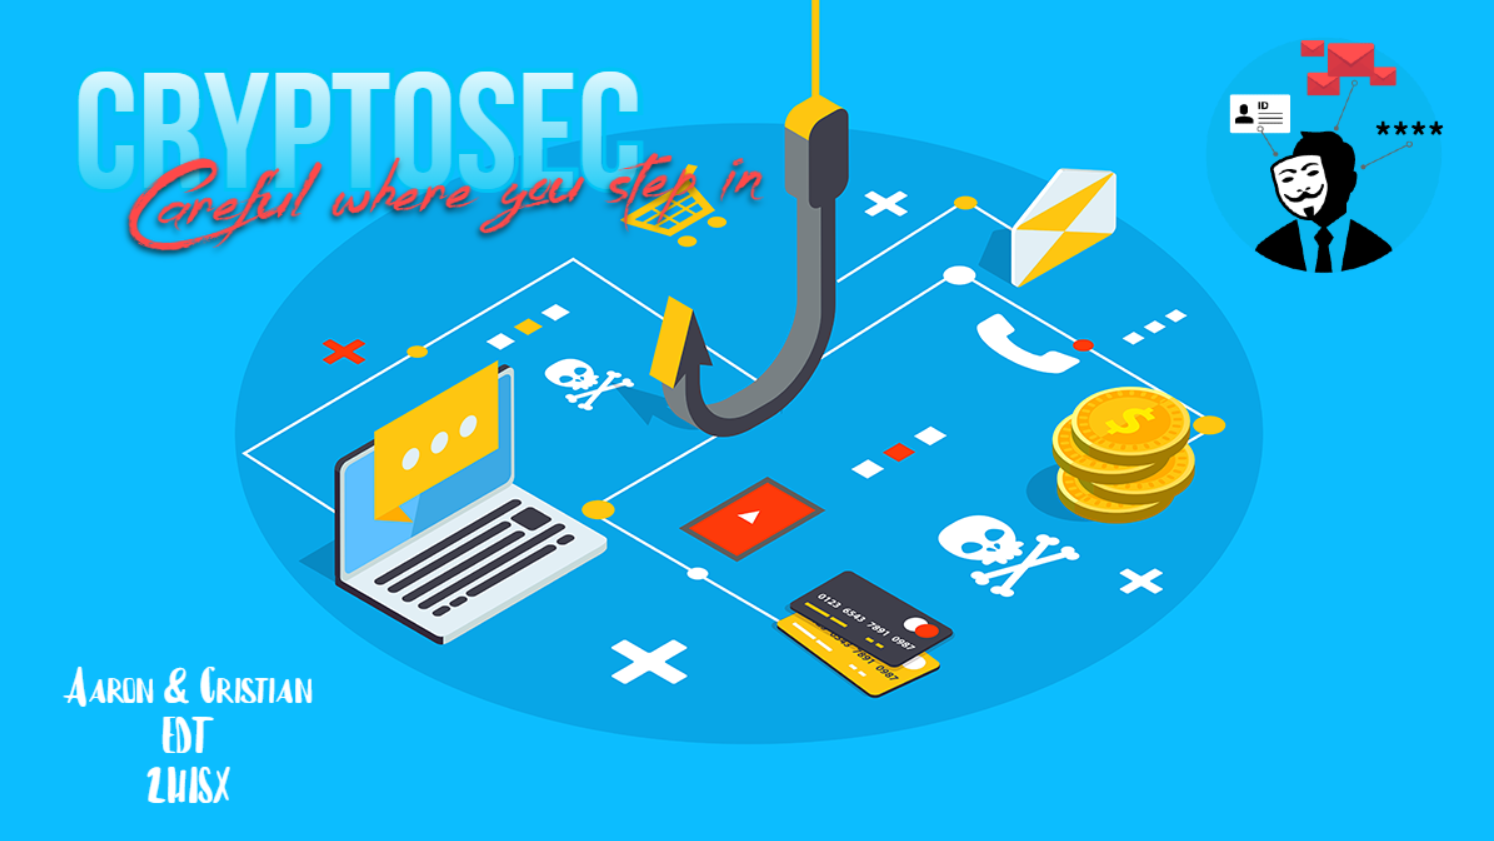
\includegraphics{./tex2pdf.-b3b523b39f59cb58/785b57206d80bd3d5ef15f036481e103db8435a1.png}

\begin{quote}
Img src: @Aaron \& Cristian's Github
\end{quote}

\hypertarget{seguiment-asix-project-2k22---cibersegureatat-cryptosec}{%
\section{Seguiment ASIX Project 2k22 - Cibersegureatat
``CryptoSEC''}\label{seguiment-asix-project-2k22---cibersegureatat-cryptosec}}

Aquest arxiu es documentarà els passos dins del projecte que tenim al
cap.

Document els nostres moviments a petició dels professors que van
sol·licitar que ens documentéssim a nosaltres mateixos fent el projecte
final.

\hypertarget{section}{%
\subsection{19/04/2022}\label{section}}

Cristian= 08:45-13:55 (2h)

Busca informació sobre el sistema de detecció d'intrusió, Wazuh i les
seves característiques a diversos llocs per Internet. Mirant diversos
exemples de presentacions de projectes relacionats amb el nostre, per
agafar idees dels nostres objectius.

\hypertarget{section-1}{%
\subsection{20/04/2022}\label{section-1}}

Cristian \& Aaron = 19:45-21:50 (3h)

Planificant els seus objectius de treball pel projecte, organitzant les
ideés i començant a les preparacions. I fent un esborrany d'un esquema
improvisat sobre la nostra idea.

Comencen per muntar Docker: un implementat amb WireGuard VPN i l'altre
amb DNS. A manera de prova, testegem amb el Packet Tracer l'esquema
improvisat.

Continuant ampliant les nostres idees, ajuntant WireGuard amb Wazuh (o
Radius) i iptables. Al DNS criptogràfic l'hi afegirem Open SSL amb un
parell de claus privades. Hem decidit afegir un Docker més: aquest
tindrà dins \ldots{}

Passen omplir la introducció del nostre projecte, buscant informació
sobre la ciberseguretat. Ficant múltiples definicions i imatges.

\hypertarget{section-2}{%
\subsection{25/04/2022}\label{section-2}}

Aaron=8:55-10:45 (2h)

Organitza els documents/arxius/directoris dins del git del nostre
projecte (asixprojecte2k22).

Decideixo a començar a indagar sobre el DNS Criptography, entendre
millor el que és, com funciona, quines capacitats ofereix el DNS.

Posa en pràctica un DNS Criptography a una màquina virtual (VirtualBox).

Cristian=8:00-13:10 (3h)

Continua buscant dades sobre el Wazuh i sobre les seves capacitats que
ofereix com a sistema de detecció d'intrusions.

Busca una pràctica amb què intenta posar en marxa per aprendre més sobre
Wazuh.

Cristian \& Aaron = 16:00-19:45 (3h)

Segueixen omplin els Objetius, el Seguiment i despres segueixen buscant
informacion sobre DNS Criptography i començant una practica de Wazuh.

\hypertarget{section-3}{%
\subsection{26/04/2022}\label{section-3}}

Cristian \& Aaron = 12:10 - 14:00

Monten un tant un Linux Lite i un Ubuntu Server dins de VirtualBox.

Com Aaron i en Cristian tenen Windows a casa han optat per una full
virtualization d'un o varies Ubuntu Servers a VirtualBox. Per aquest
motiu el format del fitxer vdi (virtualbox disk) és portable i podem
avançar a casa. L'accés i configuració es farà per ssh amb un parell de
claus pub/priv.

La instal·lació es farà des de zero amb un disk iso de ubuntu server
20.04 i allà instal·larem els serveis quan ens hagi funcionat.

\begin{figure}
\centering
\includegraphics{./tex2pdf.-b3b523b39f59cb58/98ddfaf6f0d21012a23616a25ca441e036a8cd13.png}
\caption{Llegir}
\end{figure}

\hypertarget{section-4}{%
\subsection{27/04/2022}\label{section-4}}

Cristian \& Aaron = 9:00 - 12:00

Research d'esquemes i tipus d'atacs per al projecte. Ordenació del GIT
del projecte. Instal·lació i pre configuració d'Ubuntu Server a Virtual
Box. Tenir una idea definitiva i separar diferents pràctiques per a la
posterior assemblatge.

\hypertarget{section-5}{%
\subsection{28/04/2022}\label{section-5}}

Aaron = 18:00 - 20:00

Configuració de les màquines virtuals Ubuntu Server i clients Ubuntu i
Debian 10 a VirtualBox.

Bases de proves de diferents atacs informàtics com ARP Spoofing o DNS
Poisoning. També KeyLoggers i atacs d'Enginyeria Social.

Muntatge sobre Kali Linux (Atacant) i un servidor d'Ubuntu Server 20.04
i un client Debian Minimal.

\hypertarget{section-6}{%
\subsection{02/05/2022}\label{section-6}}

Aaron \& Cristian = 09:00 - 14:00 // 15:00 - 19:00

Research d'informació dels diferents atacs informàtics. I bases de
proves en les nostres màquines.

Proves a Kali Linux de les diferents atacs informàtics.

Proves de Man in The Middle Attack, DNS Spoofing, atac d'Enginyeria
Social, ARP Spoofing.

\hypertarget{section-7}{%
\subsection{03/05/2022}\label{section-7}}

Aaron \& Cristian = 09:00 - 14:00

Proves finalitzades: atac d'Enginyeria Social amb imatge QR Research
d'informació dels diferents atacs informàtics. I bases de proves en les
nostres màquines.

Continuació de les proves de Man in The Middle Attack, ARP Spoofing i
Keylogger Aaron fa proves de DNS Cache Poisoning amb Kali Linux i
Cristian fa un esquema del projecte mentres prova un KeyLogger a Windows
desde Kali Linux.

Aaron fa proves de DNS Cache Poisoning. Cristian reserca sobre mes prove
practica de keyloggers.

\hypertarget{section-8}{%
\subsection{04/05/2022}\label{section-8}}

( Aaron \& Cristian = 08:00 - 12:00

Cristian estaba fent una última prova de Windows 10 amb el KeyLogger.
Pero per raons que desconèixem i per part de Windows no ha funcionat.
Pero ho ha documentat tot correctament a la carpeta de KeyLogger.

Aaron, estaba revisant i documentat DNS Cache Poisoning / DNS Spoofing i
ARP Spoofing també fent proves amb el Kali Linux. A l'hora del Gerard,
va sortir correctament el Toolkit que vam provar per fer l'atac per
``robar'' les credencials de una víctima host.

La victima host posa www.twitter.com i es redirigeix a una web falsa que
hem clonejat anteriorment, igual que twitter. Un cop posa l'usuari i
password, tenim un programa anomenat Ettercap que esnifarà el resultat
d'aquest atac.

Proves finalitzades: atac d'Enginyeria Social amb imatge QR Research
d'informació dels diferents atacs informàtics. I bases de proves en les
nostres màquines. DNS Spoofing + ARP Spoofing --\textgreater{} Accés a
Twitter.

Després Cristian va estar buscant informació de DNSSEC.

Copies de seguretat de les màquines VDI.

\hypertarget{section-9}{%
\subsection{05/05/2022}\label{section-9}}

Aaron \& Cristian = 09:00 - 12:00

Aaron termina de repetir el procés d'ahir amb captures i entendre el
resultat.

Cristian fa el muntatge de DNSSEC.

\hypertarget{section-10}{%
\subsection{06/05/2022}\label{section-10}}

Aaron \& Cristian = 10:00 - 12:00

Aaron fa la exhibició de Kali Linux de DNS Spoofing y ARP Spoofing per
suplantar www.twitter.com i la suplantació del reenviament de paquets
entre una connexió Client-Servidor a Eduard Canet.

Cristian segueix buscant DNSSEC.

\hypertarget{section-11}{%
\subsection{09/05/2022}\label{section-11}}

Aaron \& Cristian = 08:00 - 14:00 ; 16:30 - 21:00

Cristian fa la implementació de DNSSec a Ubuntu Server mentres que Aaron
fa més research de Kali Linux, de les eines que ha utilitzat, tot i fent
la documentació adhient.

Aaron ha intentat un altre atac, que es desencriptar contrasenyes
SHA-512 Unix amb una eina de Kali.

Cristian implementa el DNSSec, documentat, falta base de proves.

Proves en la tarda de DNSSEC OK. Amb la comanda dnssec-signed creem un
fitxer firmat de la nostra zona db.cryptosec.net.signed i en
funcionament OK.

\hypertarget{section-12}{%
\subsection{10/05/2022}\label{section-12}}

Aaron \& Cristian = 08:00 - 14:00

Cristian ha continuat amb la practica DNSSEC, ha porvat dues formes de
signatura.

L'Aaron ha fet una recerca d'informació de DNS, partint de la base i
refrescant conceptes com DNS Recursiu, DNS TLD, Root Servers, DNS
Forwarding\ldots{} Exemples i terminologies i conceptes varis de DNS.

Quan sapiguem la base d'ambdues cosas farem exemples de DNS adaptades a
la nostra organització o zona ``Cryptosec.net'' i farem un intent d'atac
de DNS Sense DNSSEC i després implantació de DNS Segur i veurem com
procesa l'un i l'altra.

Aaron \& Cristian = 18:00 - 20:20

Han continuat amb les seves recerques, es posible que acabin dema.

\hypertarget{section-13}{%
\subsection{11/05/2022}\label{section-13}}

Aaron \& Cristian = 08:00 - 12:00

Amb l'ajuda d'en Gerard, hem reconfigurat el nostre esquema de
Ciberseguretat implantant un altre servidor que serà Forwarder al DNS
SOA autoritatiu original, rebrà les peticions. L'atac es farà al
forwarder.

Es farà un exemple de DNS sense Sec i un DNSSEC.

Aaron = 18:00 - 19:30

Aaron retoca i passa algunes coses a net en el GIT del Projecte. Canvia
l'objectiu entre altres coses.

\hypertarget{section-14}{%
\subsection{12/05/2022}\label{section-14}}

Aaron \& Cristian = 09:00 - 12:00

Aaron i Cristian fan el muntatge de les peçes del projecte configurant
DNS amb el altre servidor DNS Forwarder i el Debian Minimal com a
client.

Aaron = 15:00 - 19:00 ; 20:00 - 00:00

Aaron fa l'arquitectura de CryptoSEC implementant el DHCP per a que el
client DEBIAN de la nostra Xarxa Interna tigui una IP DINAMICA assignada
per el SOA.

Fa proves amb el Kali Linux muntant tot lo que hem recapitulat fins ara,
provant amb el SET el SPOOFING i Clonatge de pàgines WEB per poder fer
la suplantació.

Automatització mitjançant IPTABLEs per a la gestió de SSH a KALI o al
RECURSOR.

Implementació de DHCP amb DNS resolv automàtic per als clients de
Cryptosec.

Més proves i passar a net la documentació.

Aaron

\hypertarget{section-15}{%
\subsection{13/05/2022}\label{section-15}}

Aaron \& Cristian = 11:15 - 12:00

Aaron i Cristian fan de nou l'esquema modificant coses de l'arquitectura

Aaron = 15:00 - 17:30

Aaron implanta un Apache2 amb una plantilla d'un formulari amb HTML i
CSS per posar-ho a www.cryptosec.net, els habilita amb a2ensite. Tant
HTTP 80 com HTTPS amb SSL 443.

Amb KALI prova alguna pàgina de bancs. Funciona Banc Sabadell.

Aaron = 19:20 - 00:30

Aaron segueix fent proves amb el Kali i fent una demo a Cristian, seguim
construint DNSSEC.

\hypertarget{section-16}{%
\subsection{16/05/2022}\label{section-16}}

Aaron \& Cristian = 08:00 - 13:00

Aaron parla amb el Gerard i modifica tot l'arquitectura de CryptoSEC.
L'atacant Kali provindrà de la CLASSE.

Tindrem un Forwarder-Recursiu que serà un DNS Forwarder a un SOA. El soa
tindrà una zona coneguda com DNS Primary un SOA ``cryptosec.net''.
S'allotjarà un Web Server Apache2 que tindrà una pàgina d'exemple.

Seguint fent l'assemblatge.

Aaron i Cristian = 16:00 - 20:00

Demo i terminar coses pendents. Temes d'atacs, DNSSEC, crackets (brute
force), ssltrip \ldots{} etc.

S'ha de terminar de documentar i passar a net.

\hypertarget{section-17}{%
\subsection{17/05/2022}\label{section-17}}

Aaron \& Cristian = 08:00 - 13:00

Un nou deployment s'ha presentat i s'ha modificat tot l'esquema de
CryptoSEC.

S'ha instal·lar al SOA un Apache2 amb una pàgina de template.

Aaron i Cristian = 16:00 - 20:00)

Revisar la doc i ordenar el GIT del projecte.

\hypertarget{section-18}{%
\subsection{18/05/2022}\label{section-18}}

Aaron \& Cristian = 08:00 - 13:00

Practica la demo i practicar amb el Kali els diferents tipus d'atacs.
Seguint practicant amb el Ettercap i el \textbf{site cloning}.

Modificar les pàgines per Kali que s'utilitzaràn per a la demo de DNS
Spoof.

\hypertarget{section-19}{%
\subsection{19/05/2022}\label{section-19}}

Aaron \& Cristian = 08:00 - 21:00

Últimes pràctices abans de presentar el dilluns, es descobreix l'ús de
Bettercap i Zphishing, eines potents per a fer MITM.

Es continua documentat tot el procediment.

Es segueix practicant per a la demo final.

\textbf{Atacs finals}

Brute Force Attack - Cracking Password with John: El hacker ha
aconseguit una copia dels fitxers /etc/passwd i /etc/shadow i les ha
anomenat mini-passwd.txt i mini-shadow.txt. John és un tool de Kali que
permetrà desxifrar els hashes de les contrasenyes. Quant més difícil més
temps trigarà. Posarem contrasenyes sencilletes. Podrem veure com les
desxifra. Utilitzarà un diccionari rockyou.txt. Aprofitant també que
l'usuari ha

ARP Poisoning / Spoofing (2 parts) (BETTERCAP): Envenenament de les
taules ARP de les víctimes implicades i reenviament de paquets al
hacker. Amb el Wireshark - ARP - Nmap, veurem com fa el duplicat de MAC.

MITM - Eavesdropping (Sniffing) (BETTERCAP): Amb l'ARP Spoof d'abans
activarem un sniffer i estarem escoltant la màquina afectada i veient
les pàgines on visita. Podem captar credencials de pàgines HTTP.

DNS Poisoning / Spoofing) (BETTERCAP): Amb l'ARP Spoof d'abans activarem
un dnsspoof i injectarem un registre de DNS fals on ens redirigirà a la
nostra màquina on hi tindrem una fake page: m0odle.escoladeltreball.org
(Moodle EDT) i l'enviarem per correu utilitzant SET dient que ``URGENT!
L'Eduard ha posat les notes de M06, entra urgentment i mira la nota que
tens!!!'' llavors l'usuari entrarà i no se n'adonarà i li robarem les
credencials mostrades al SET.

Spoofing CryptoSEC.NET + DOS SlowHTTP (take down cryptosec.net)
(BETTERCAP): Ídem que l'anterior, però els targets son el SOA i el
Forwarding, els clients interns de CryptoSEC quan hagin d'anar a la
pàgina web cryptosec.net, entraràn a cryptos3c.net ja que el hacker ha
avisat que hi hà una urgència a la pàgina principal i han d'entrar a la
pàgina web dada pel hacker i les seves credencials seràn robades sense
que se n'adoni! Abans de tot, el hacker utilitzarà una eina perquè la
pàgina de cryptosec.net vagi més lent durant uns minuts. Durant aquest
minut aprofitarà per donar un comunicat oficial a l'empresa CryptoSEC
dient que la pàgina ha sigut tumbada i han d'anar a una altra anomenada
cryptos3c.net.

ZPHISHING: Phishing with a real ``fake'' HTTPS website: Exemple real de
Phishing automatitzat i desplegat a Cloudflare per un programa anomenat
Zphishing. Genera servidor temporal a Internet amb una plantilla a
escollir de l'usuari. Enmascarar l'enllaç amb un url shortner i
enviar-ho a alguna víctima mitjançant SET que enviarà el correu
automàticament amb un compte de Gmail. L'usuari entrarà, però no veurà
l'enllaç perquè és una emergència i posarà les seves credencials.
D'aquesta manera recollirem l'usuari i la contrasenya de l'usuari
(Credential Harvester).

\hypertarget{section-20}{%
\subsection{21/05/2022}\label{section-20}}

Aaron \& Cristian = 09:00 - 21:00 )

Revisió de la documentació i practicar els diferents tipus d'atacs que
hem estat desplegant al llarg d'aquest temps.

Recerca d'informació, es descarten algunes opcions ja que no han acabat
de funcionar o bé estaven incompletes.

\hypertarget{section-21}{%
\subsection{20/05/2022}\label{section-21}}

Aaron \& Cristian = 14:00 - 21:00

Passar a net la presentació i creaació del \emph{slidy}

Aaron i Cristian = 16:00 - 20:00

Demo i terminar coses pendents. Temes d'atacs, DNSSEC, crackets (brute
force), ssltrip \ldots{} etc. Seguint practicant per a la demo i
actualització dels atacs i posterior documentació a net.

Video d'1 minut del projecte \emph{done}.

\hypertarget{section-22}{%
\subsection{21/05/2022}\label{section-22}}

Aaron \& Cristian = 10:00 - 13:00

Seguint fent proves amb Kali, es descobreix més atacs com el DOS per
atacar cryptosec.net.

Seguir passant la informació a net.

Aaron i Cristian = 14:00 - 20:00

Demo i terminar coses pendents. Temes d'atacs, DNSSEC, crackets (brute
force), ssltrip \ldots{} etc.

S'ha de terminar de documentar i passar a net.

\hypertarget{section-23}{%
\subsection{22/05/2022}\label{section-23}}

Aaron \& Cristian = 08:00 - 13:00 )

Assaig i verificació del contingut del projecte

Aaron i Cristian = 16:00 - 20:00)

Demo i terminar coses pendents. Temes d'atacs, DNSSEC, crackets (brute
force), ssltrip \ldots{} etc.

S'ha de terminar de documentar i passar a net.

\hypertarget{section-24}{%
\subsection{23/05/2022}\label{section-24}}

Aaron \& Cristian = 09:00 - 18:00 )

Presentació final del projecte amb demostracions.

Passar a net i corregir erros de la documentació.

Penjat el video\ldots{} etc.

Tot correcte. Documentació \emph{done}.

\end{document}
